\iffalse
{Oliver Kopp, Marcel~Kr\"uger, Marei~Peischl}
{Tutorial: Creation of \LaTeX\ documents using a cloud-based pipeline}
{This will be a tutorial on using git as well as GitHub\slash GitLab
pipelines for \LaTeX\ document development. The duration is expected to
be two hours or more, depending on the final schedule.

Most \LaTeX{} users compile on the local machine or using online
services like Overleaf. There also is a third option: build servers.
That option is especially interesting when one versions the project
using git. This tutorial will show you how to get from an installation
of git to a \LaTeX\ document compiled by a build server. At first,
concepts of git and GitHub\slash GitLab will be explained. This includes
the concept of branches, pushes, automated checks on the build server,
and collaborative work using pull\slash merge requests. After that,
there will be time for practical exercises and questions.

Participants are asked to create a GitHub or GitLab account before the
start, but we will also show how to run a pipeline locally so this is
not a strict requirement.}
\fi

\documentclass[final]{ltugboat}
\def\ldots{\tubdots\allowbreak}
\PassOptionsToPackage{draft}{minted}

\usepackage{Peischl_expl3tut-config}
\usepackage{microtype}
\usepackage{graphicx}
\usepackage[hidelinks,pdfa]{hyperref}
\usepackage[autostyle]{csquotes}


\usepackage{biblatex}
\addbibresource{tug2024-cicd.bib}

\usepackage{tabularx}
%%% Start of metadata %%%

\title[TUG2024: LaTeX CI/CD]{Tutorial:\newline Creation of \LaTeX\ documents using a cloud-based pipeline}
\date{2024-07-19}

% repeat info for each author; comment out items that don't apply.
\author{Marei Peischl}
\address{Gneisenaustr. 18\\20253 Hamburg\\Germany}
\netaddress{marei (at) peitex dot de}
\personalURL{https://peitex.de}
%\ORCID{0}
% To receive a physical copy of the TUGboat issue, please include the
% mailing address we should use, as a comment if you prefer it not be printed.
\author{Marcel Krüger}
\address{Gneisenaustr. 18\\20253 Hamburg\\Germany}
\netaddress{marei (at) peitex dot de}
\personalURL{https://peitex.de}
\author{Oliver Kopp}
\address{Gneisenaustr. 18\\20253 Hamburg\\Germany}
\netaddress{marei (at) peitex dot de}
\personalURL{https://peitex.de}

%%% End of metadata %%%
%\addbibresource{dante-expl3tut.bib}       % xampl.bib comes with BibTeX}

\newif\ifTUGboatPrint

\TUGboatPrinttrue

%black & white mode for printing
\ifTUGboatPrint
\usemintedstyle{bw}
\AtBeginEnvironment{minted}{\let\textit\textsl\let\itshape\slshape}
\AtBeginEnvironment{tcolorbox}{\let\textit\textsl\let\itshape\slshape}
\tcbset{
	MintedFunctionframe/.append style={
		before upper={\let\textit\textsl\let\itshape\slshape}
	}
}
%These are the background colors of the boxes
\colorlet{CommentColBack}{black!2}
\colorlet{ListingColBack}{black!8}
\colorlet{TextColBack}{black!4}
\colorlet{TitleColBack}{white}
\fi

\usepackage{hologo}
\expandafter\def\csname HoLogo@TeX Live\endcsname{
	\TeX\,Live
}

\newcommand*{\TeXLive}{\acro{\TeX\,Live}}



\usepackage{fontspec}

\directlua{luaotfload.add_fallback
("emojifallback",
	{"NotoColorEmoji:mode=harf"}
)}

\setmonofont{Latin Modern Mono}[RawFeature={fallback=emojifallback}]

\newcommand*{\action}[1]{\texttt{#1}}
\newcommand*{\command}[1]{\texttt{#1}}
\newcommand*{\directive}[1]{\textbf{\detokenize{#1}}}
\newcommand*{\file}[1]{\texttt{#1}}
\newcommand*{\directory}[1]{\texttt{#1}}
\newcommand*{\containerimage}[1]{\enquote{#1}}

\graphicspath{{}{img/}}

%TODO acro
% cici = continous ingegration and continous delivery
\begin{document}

\newlength{\mintednumbersep}
\sbox0{\tiny00}%
\setlength\mintednumbersep{1em}%
\addtolength\mintednumbersep{-\wd0}%
\setminted{xleftmargin=1em,numbersep=\mintednumbersep,numbers=left}

\maketitle

Everything went into or is moving towards the cloud.
\LaTeX{} is already there for about 10 years and today it's quite common to use a web editor for collaboration and local compilation became the \enquote{nerdy} way.
But there also is a third variant to compile documents which can be used also to improve package development and in general the stability of \LaTeX{}:
Adapting DevOps methods, like \acro{CI/CD} for the workflow and compiling using automated workflows.

\section{Why should I?}
Having some working workflows usually makes people to not think about changing anything.
So there have to be reasons why it might be worth reading this article or even integrating the mechanisms into projects.

Originally the idea was to folliw the current state of OpenSource development and open a door for contributors in the development process,
For example the \LaTeX{} Project is currently creating a lot of user interaction via their GitHub projects~\cite{latex3-github} and also taking contributions from which the whole \TeX/\LaTeX{} community will profit.

But the advantages of these methods go even further\footnote{We focus on some aspects as this could probably male an article by itself.}

\subsection{Works for me?!}
Sometimes compilation failes on some systems, but doesn't on others.
This may have tons of reasons so having some pipeline configured will show if this a machine specific issue or a general one.

\subsection{Compatibility and regression testing}
It's possible to run the workflow on multiple TeX distributions or versions.
This can be used to know if there are any issue with some package update before the actual update where downgrading may be complicated\footnote{That's another issue to address … but a differen story.}

Additionally you can also use it to check backwards compatibility e.\,g. if one collaborator is using a Debian Stable which is stuck on some outdated version.
As mentioned the \LaTeX{} Project Team is already using this techniques and even provides functionality for regression testing within their build system \enquote{l3build} \cite{l3build}.

Using this as a package developer enables a general interface to be used for regression testing.
This allows to avoid some of the bugs which otherwhise would be published and should be found by a user.
Also it can be used to avoid inconsitent structures, e.\,g. one of the authors recently found that tons of packages and files within \TeXLive{} don't have a proper version number set within the code.

\section{Structure of this tutorial}

The idea is to introduce readers to the basics of setting up automated workflows on GitLab, GitHub or Forgejo.

This tutorial mainly addresses two groups of users:

\begin{enumerate}
\item Authors which focus on typesetting actual content. This includes collaborations.
\item Package or template developers, who provide their work to be used by the first group.
\end{enumerate}

The second group obviously can also  use workflows of the first e,g, for typesetting documentation.
So developers usually use an extended version of the the setup provided for the authors.

As all used platforms usually are used to be used with git we expect the project to be some kind of git repository.
In case the reader does not yet use git, there is a little bit of information attached to this tutorial.
Using that it would be possible to use git without even noticing as it's attached to the autosave function of an editor.

As the \LaTeX{} project is using GitHub this is how we are going to start with detailed explanation and afterwards will create a matching setup on the other platforms.
There have been example repositiories created which can be used as a template.

The explanations within the GitHub section are a bit more detailed.
It is planned to have some extended version of this article where instructions are only focusing on the specific platform.

\section{Compiling a document in a CI pipeline}

\subsection{First steps with GitHub Actions}

To get started we need a git repository somehow hosted GutHub.
May also be a private one.

Thinking of the tasks we have to resolve there will be:

\begin{enumerate}
\item Prepare the environment to have some \LaTeX{} distribution
\item Run \LaTeX{}
\end{enumerate}
%
\noindent GitHub is providing pre-configured actions which are able to combine multiple steps, e.\,g. the latex-action \cite{latex-action}.
This  is starting another container inside the action container to run latexmk.
But those actions usually limit the configuration options to simplify the interface.
We are going to checkout both variants.

The configuration for an action is done by creating a yaml file within the repositories subdirectory \file{.github/workflows/hellow-world.yml}.
The name may be choosen individually.
The following code snipped shows a minimal configuration:

%\begin{listing}
\inputminted{yaml}{examples/hello-world.yml}
%\caption{ \file{.github/workflows/build.yml} directly using a LaTeX action}
% \label{list:hello-world}
%\end{listing}

\begin{description}
\item[name:] of the workflow.
This is important if a project contains multiple workflows.

\item[on:] This directive selects when the workflow should be started.
This setting means it will be started on any push. So whenever the repository on the server receives an update.

\item[jobs] contans a list of jobs to be run after each other.
For example it's quite common to have one for testing and one for deployment.
In this example it only contains one job called \enquote{action-test}.

\item[runs-on:] the value corresponds to a runner setup.
Runners are the machines to actually run the workflow.
It doesn't have to be the same server as the one where the repository is hosted.
In the example \enquote{ubuntu-latest} is chosen.
This is one of the provided runners by GitHub which is based on ubuntu.
It includes nodejs and some tooling to simplify the work using predefned actions.
A full list of the runners and detailed description of the images can be found at cite{github-hosted-runners}.

\item[steps:] This is what the workflow should actually do.
As one can see it's possible to directly enter bash code in there.
This example is only creating some output and should therefore run without any issues.
\end{description}

On GitHub the actions are automatically enabled.
So it's enough to add a yaml configuration file within the repository and since we chose one of the runner variants which are also provided by Github, no additional setup is required.
The pipelie should start running.

The status can always be checked having a look at
\url*{<repo url>/actions} e.g. for for first of our demo repositories, this can be found at
\citefield{workflow-github}{url}/actions.%TODO url - needs expansion

\noindent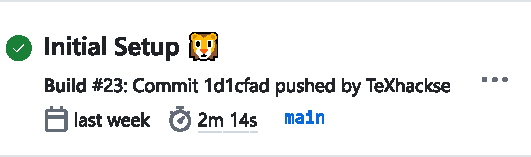
\includegraphics[width=\linewidth]{screenshot-pipeline-successful}

The pipeline run successful but did not anything but create some shell output.
So next step is to move towards \LaTeX{} usage.

\subsubsection{Actually using \LaTeX}

As already mentioned actions are mostly based on docker.
Luckily some of the us live on the Island of TeX and prepare some images we could make use of here\footnote{Special thanks to the other islanders at that point!}.
The setup of the images was described within \cite{islandoftex-docker-gitlab}.

The first part of the workflow will stay the same for the moment.
Changes only apply after `runs-on`:

\inputminted[firstline=5, lastline=12,gobble=3]{yaml}{examples/latex-basic.yml}


\begin{description}
\item[container:] Choosing the IoT \containerimage{texlive-latest} image which provides a full TeX Live + some tools\cite{islandoftex-docker}.
\item[steps:]
The first step looks different from the one, we had before.
It received a name, which is helpful to simplify debugging as GitHub will tell us which step failed.

\item[uses:] is a reference to another action.
Github uses this to have some kind of interface for pre-configured pipelines as there are tasks which are more complex than it seems.
So \action{checkout@v4} refers to a separate repository \cite{github-action-checkout}.
This action is taking care of the authentication and some interals, so we don't have to deal with details.

Important is, that after this action the following steps start being executed within the root directory of our repository.

The second step is kind of the same as in the first example, but this time we run \command{latexmk}\cite{latexmk} using \command{lualatex}.
By default this will run on all \file{*.tex} files within the root directory.
So we don't even have to depend on the file name as long as we store files to be included within subdirectories.
\end{description}

\subsubsection{Where's the PDF?}
If the pipeline run successfull there will be a green checkmark but we will fail finding the PDF somewhere.
This is because GitHub does not yet know which files actually are the output which should be kept.
Such files are called \enquote{artifacts}, so now it should be added to keep the PDF as such and upload that one to GitHub.

\inputminted[firstline=13, lastline=17,gobble=3]{yaml}{examples/latex-basic.yml}

After another (successful) run of the pipeline it's possible to access the pdf wrapped within a  \file{*.zip} at the run's status page.
Clicking on the run on the actions overview page leads there:

<include image of the artifact>

Sadly GitHub is currently does not provide an option for individual files without a zip.
Also it's not possible to have a static link pointing to the latest artifacts.
Other plattforms like Gitlab do provide that feature by default.
To resolve and make the pdf easier to access on GitHub it's required to use additional actions.
The most common way to do it is publishing the pdf an orphan branch.
Usually this mechanism is used to create web pages and is called github-pages.

<insert listing>

\subsection{Differences with actions on Forgejo}
Forgejo\cite{forgejo} is another code plattform which has the aim to be more open than GitHub.
It can be self-hosted and now provides mechanism similar got GitHub actions.

They will never completly do the same as GitHub does, but they are almost compatible.

By default Forgejo will search within \directory{.forgejo/workflows/} for configuration files.
If none are found it will even fall back to look inside the \directory{.github/} directory.
Only issue would probably face is that there are no hosted runners on most instances.
And in case there are they will probably be different from GitHub's.

But in case you can configure a runner yourself and use the labels as the GitHub runner \cite[described in]{forgejo-runner-config} was using it's possible to use the same workflow configs on both.
The provided demo repositories on codeberg.org, which is a Forgejo instance, also explain how the runners used there are configured.

\subsection{Compiling a document using GitLab CI}

Gitlab is not that much different. Actually it's a bit easier to use here as it provides some features automatically.
For example it's not necessary to checkout into the repository.
That's already done by default.

\inputminted[breaklines,breakafter=/]{yaml}{examples/latex-basic-gitlab.yml}

Here the steps only are a list of commands run after each other. Currently the list only contains one \command{latexmk} call.

As mentioned before Gitlab is providing an API which allows to create static links to the artifacts.
So the \file{README.md} of the demo repositories there include a link of the following structure:

<Link to Gitlab Repo>/-/jobs/artifacts/<branch>/browse?job=<name of the job>

this will list all artifacts attached to the job.
Using the example config on one of the demo projects would make it

\citefield{workflow-document-gitlab}{url}/-/jobs/artifacts/main/browse?job=run-LaTeX

\section{Testing with multiple versions or compilers}

We promised one can extend these setups to test using multiple versions or compilers.
Different compilers are actually sraightforward by including additional steps running different commands.
Of course it's possible to use those in separate actions or even workflow files.
There is no general way to strucure those, as it always depends on if they all should always run or better depend on each other to save resources.

For using other versions of \TeXLive{} the IoT is providing historic images.

\begin{minted}[escapeinside=||,breaklines,breakafter=/]{yaml}
test-on-IoT-texlive:
  runs-on: ubuntu-22.04
  strategy:
    matrix:
      image: ["TL2022-historic", |…|]
  name: "Test on ${{ matrix.image }}"
  container:
    image: registry.gitlab.com/islandoftex/images/texlive:${{ matrix.image }}
  steps:
\end{minted}

\begin{description}
\item[strategy:] this is used to create a loop over elements.
In this case a variable called \mintinline{yaml}|matrix| containing a list of images is used and the content can be accessed within other parts of the file using \mintinline{yaml}|${{ matrix.image }}|.
So the first run will be on \enquote{texlive:TL2022-hostoric}.
A full list of the provided images can be found at \cite{islandoftex-docker-gitlab}.
\end{description}

For Gitlab again the structure is similar but not matching:

\begin{minted}[escapeinside=||,breaklines,breakafter=/]{yaml}
check:
  image: registry.gitlab.com/islandoftex/images/texlive:$TEXLIVE_VERSION
 |[… contains script + artifacts … ]|
  parallel:
    matrix:
      - TEXLIVE_VERSION: ['TL2022-historic', 'TL2023-historic', 'latest']
        TEX_ENGINE: ['pdflatex', 'xelatex', 'lualatex']
\end{minted}

Here the variable is more like a bash variable but can be used the same way.


\section{Minimize the build container}
We currently use a full TeX Live installation to have the most convenient setup.
The IoT Images even support additional tools like arara or minted.
But sometimes it might be useful to minimize the build container, either because downloads take too long or we have limited space available on the runner server or just to save resources.

The most annoying part here might be to find out which packages are actually needed to compile…

So… the Island of TeX proudly presents: DEPP – The DEPendency Printer for \TeXLive\cite{depp}

As this article should focus on pipelines we won't go into detail, but the idea is that DEPP is producing a file listing all TeX Live packages necessary for the build.
For the example projects these look like:

\begin{minted}[breaklines,escapeinside=||,linenos=false]{text}
#Proudly generated by the Island of TeX's |[…]|
blindtext
cm
|…|
\end{minted}

\subsection{GitHub}

On Github there are two actions installing TeX Live as a part of the workflow.
Using those it's possible to minimize the container and this will also reduce the build time.

\begin{minted}{yaml}
- name: Install TeX Live
        uses: zauguin/install-texlive@v3
        with:
          package_file: .github/tl_packages
\end{minted}

This snippet can be used within \directive{steps:} and makes the \directive{container:} directive to be obsolete, so it should be removed.
The \directive{package_file:} is the path to the DEPP-output or some manually created list of packages.

 \subsection{GitLab}

 On Gitlab the simplified syntax makes this a bit more complex.
 The DEPP repository is luckily providing a shell script to install a TeX Live based on the package file.
 This can be used in the pipelines to modify the container.
 Another option would be to provide a container image which already contains the necessary packages.
 If a self hosted runner is used, this usually is the best option as caching can be configured to controll when the container is rebuilt or updated.

\section{Pipelines for package developers}

As promised the advantages or using automated pipelines are even more when used within a real development process.
In this case we expect the repository to contain a package and some kind of l3build configuration.\footnote{also works with other tools, but have to focus}

The latex or as we used latexmk command will be replaced by

\begin{minted}{yaml}
- name: Run l3build
  run: l3build check --show-log-on-error -q -H
\end{minted}

This will automatically run all testfiles according to the l3build setup.
As this is within development the artifacts are totally different.
We're not really interested in a pdf but the test output.
One of the authors created another action to take care of this:

\begin{minted}{yaml}
- name: Archive failed test output
  if: ${{ always() }}
  uses: zauguin/l3build-failure-artifacts@v1
  with:
    name: testfiles-${{ matrix.platform }}
    retention-days: 3
\end{minted}

The special about this step is, that \mintinline{yaml}|if: ${{ always() }}| has been added.
This will enforce the step to be run also if the step before failed.
As this is the case where we need it, it's necessary to add this configuration.




%\printbibliography
\def\url{\tbsurl}
\SetBibJustification{\raggedright \advance\itemsep by 1pt plus1pt minus1pt }
%\bibliographystyle{tugboat}
%\bibliography{tug2024-cicd}
\printbibliography
\makesignature




\end{document}
